\section{Answers}

\begin{enumerate}
\item Which of the following statements, regarding the usefulness of particle filters, are true?

\begin{enumerate}
\item Particle filters are useful as they can handle almost any models
\item Particle filters are useful as within reasonable computational complexity, the particle filter always gives us the best performance. 
\item Particle filters are useful as they give us a compact description of the posterior density. 
\item Particle filters are useful as they give a non-parametric description of the posterior.
\end{enumerate}

\textbf{Answer:}

The main advantage with particle filters is that they offer a non-parametric description of our posterior. As a consequence of this, it can be used to handle almost any model as long as we can evaluate them point-wise. However, it is hard to argue that we get a compact description of our posterior as we typically use a couple of thousand parameters or even more. Further, it is not a solution that should be used to solve all problems, for example, if we have linear and Gaussian models we should use the ordinary Kalman filter we know that this gives us the optimal solution. So correct options are A and D.
\item Assuming that we describe our posterior using the following approximation
\begin{equation}
p(\mathbf{x}_k | \mathbf{y}_{1:k}) \approx \sum_{i=1}^N w_{k}^{(i)} \delta (\mathbf{x}_k -\mathbf{x}_{k}^{(i)})
\end{equation}

what is the MMSE estimate of $\mathbf{x}_k$?
\begin{enumerate}
\item $\hat{\mathbf{x}}_k = \sum_{i}^{N} w_{k}^{(i)} \mathbf{x}_{k}^{(i)}$
\item $\hat{\mathbf{x}}_k = \mathbf{x}_{k}^{(j)} ~~ \text{where} ~~ j = argmax_i w_{k}^{(i)}$
\item $\hat{\mathbf{x}}_k = \frac{1}{N}\sum_{i}^{N}  \mathbf{x}_{k}^{(i)}$
\item It is not possible to calculate a MMSE estimate from this approximation. 
\end{enumerate}

\textbf{Answer:}

We can view the particle filter representation as approximating the posterior PDF with a posterior PMF where the weight, $w_{k}^{(i)}$, 
gives us the discrete probability that the state is $\mathbf{x}_{k}^{(i)}$, Using the definition of expected value on this PMF gives us the solution above. 
So the correct answer is option A.

\item Consider Figure \ref{P0_7_3_4_ex1}.

\begin{figure}[!htb]
\begin{center}
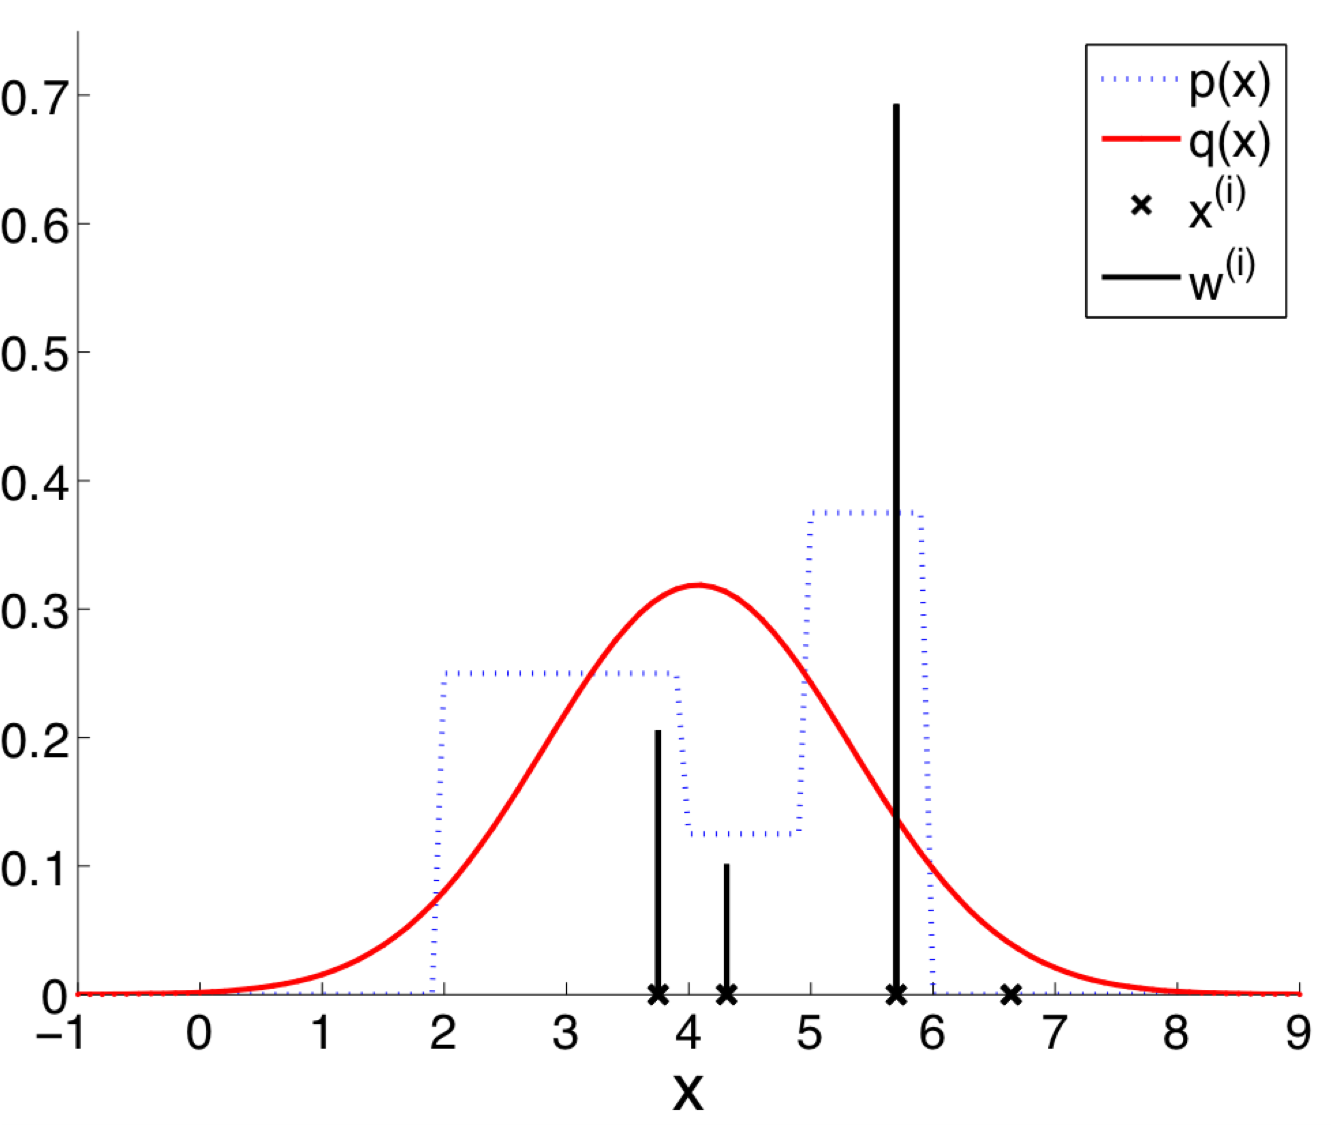
\includegraphics[scale=0.280]{img/particle_filters/P0_7_3_4_ex1.png}
\end{center}
\caption{Question figure.}
\label{P0_7_3_4_ex1}
\end{figure}
Perform resampling on the density and illustrate the result. Assume that the numbers 0.65, 0.03, 0.84 and 0.93 are drawn uniformly from $[0,1]$.
Which one of the following figures illustrates the resampled particles?

\begin{enumerate}
\item \begin{figure}[!htb]
\begin{center}
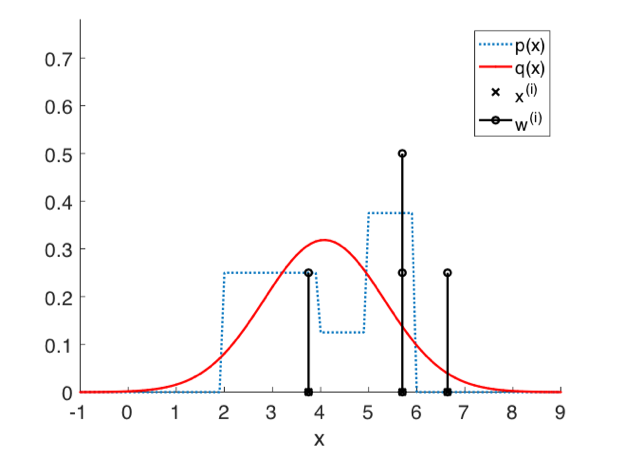
\includegraphics[scale=0.320]{img/particle_filters/P1_7_3_4_ex1.png}
\end{center}
\label{P1_7_3_4_ex1}
\end{figure}
\item \begin{figure}[!htb]
\begin{center}
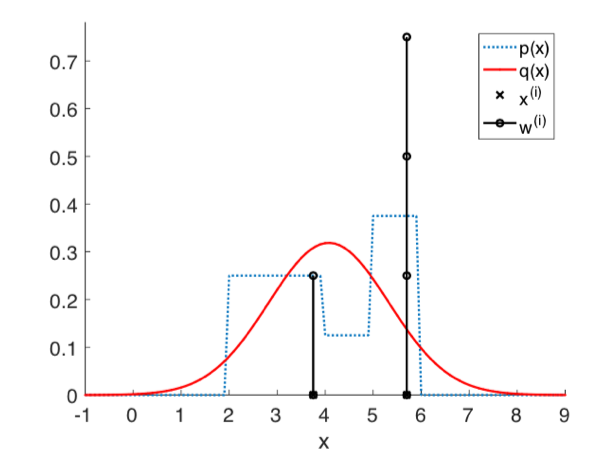
\includegraphics[scale=0.320]{img/particle_filters/P2_7_3_4_ex1.png}
\end{center}
\label{P2_7_3_4_ex1}
\end{figure}
\item \begin{figure}[!htb]
\begin{center}
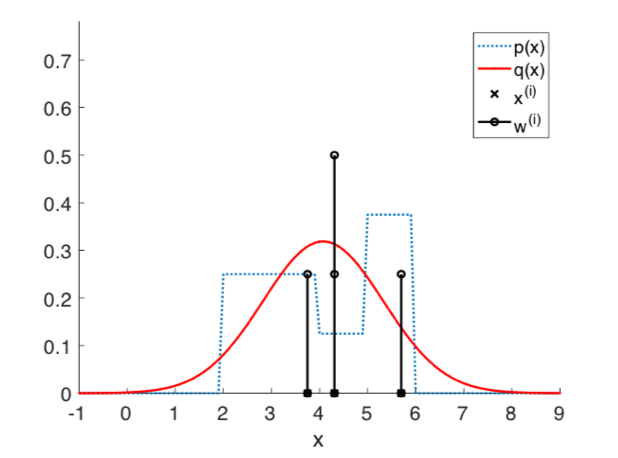
\includegraphics[scale=0.320]{img/particle_filters/P3_7_3_4_ex1.png}
\end{center}
\label{P3_7_3_4_ex1}
\end{figure}
\end{enumerate}

\textbf{Answer:}

If particles are ordered in ascending order, $x^{(1)} < \ldots < x^{(4)}$ resampling gives the following $x^{(1)} = 3.8$ and $x^{(2)} = x^{(3)} = x^{(4)} = 5.7$. Thus, option B is the correct answer.

\item Bearing only tracking with a constant velocity motion in 2D, what is $\mathbf{x}_{k}^{l}, \mathbf{u}_{k}^{l}$ and $\mathbf{y}_{k}$ in this case

\begin{enumerate}
\item $\mathbf{x}_{k}^{l}$: position, $\mathbf{u}_{k}^{l}$: velocity, $\mathbf{y}_{k}$: bearing to target
\item $\mathbf{x}_{k}^{l}$: velocity, $\mathbf{u}_{k}^{l}$: position, $\mathbf{y}_{k}$: bearing to target
\item $\mathbf{x}_{k}^{l}$: velocity, $\mathbf{u}_{k}^{l}$: bearing to target, $\mathbf{y}_{k}$: position
\end{enumerate} 

\textbf{Answer:}
Correct answer is option B. Our bearing measurements depend nonlinearly on our position state while the velocity inters linearly if we condition on the position state.



\item With the particle filters we approximate the posterior as 

\begin{equation}
p(\mathbf{x}_k | \mathbf{y}_{1:k} \approx \sum_{i=1}^{N} w_{k}^{(i)}\delta(\mathbf{x}_k - \mathbf{x}_{k}^{(i)})
\end{equation}

 Which of the following statements regarding this approximation are true?

\begin{enumerate}
\item $\mathbf{x}_k$ can take any value in $[\text{min}_i \mathbf{x}_{k}^{(i)},\text{max}_i \mathbf{x}_{k}^{(i)}]$
\item We can view this as a discrete distribution where $P(\mathbf{x}_{k} = \mathbf{x}_{k}^{(i)} | \mathbf{y}_{1:k}) = w_{k}^{(i)}$.
\item It follows that  $E[\mathbf{x}_{k} | \mathbf{y}_{1:k}] \approx \sum_{i=1}^{N} w_{k}^{(i)}\mathbf{x}_{k}^{(i)}$.
\item We can get arbitratry fine approximation by just in-creasing the number of particles, $N$ . 
\end{enumerate}

\textbf{Answer:}

Options B, C and D should be selected.

\item Consider Figure \ref{P6_importancesampling}
Which one of the Figures \ref{P6a_importancesampling}, \ref{P6b_importancesampling}, \ref{P6c_importancesampling} and \ref{P6d_importancesampling} is the importance sampling approximation of $p(x)$ using $q(x)$ ?

\textbf{Answer}

Figure C.

\item Consider Figure \ref{P7_importancesampling}
\begin{figure}[!htb]
\begin{center}
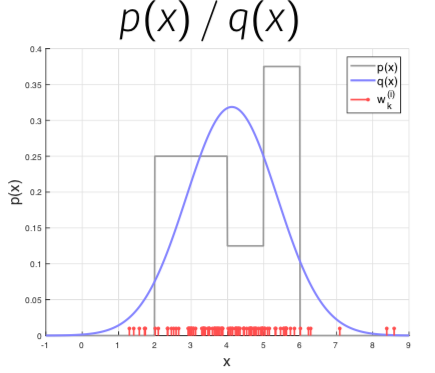
\includegraphics[scale=0.320]{img/particle_filters/P7_importancesampling.png}
\end{center}
\caption{Figure for exe}
\end{figure}

Which one of the Figures \ref{P7a_importancesampling}, \ref{P7b_importancesampling}, \ref{P7c_importancesampling} and \ref{P7d_importancesampling} is the importance sampling approximation of $p(x)$ using $q(x)$ ?

\textbf{Answer}

Figure A.

\item Which of the following is true about the SIS (Sequential Importance Sampling) particle filter?

\begin{enumerate}
\item It outputs strictly Gaussian posterior distribution approximations. 
\item It can approximate multi-modal state distributions. 
\item It eventually degenerates to just a few particles with significant weights. 
\item It is a special case of a sigma-point filter. 
\end{enumerate} 

\textbf{Answer:}

Options B and C should be selected.

\item Assume you want to compute the mean of a function $g(\mathbf{x})$ where $\mathbf{x}$ is distributed according to $p(\mathbf{x})$ which cannot
be sampled from. To compute an approximate mean, you use importance sampling with a proposal density $q(\mathbf{x})$ and the normalized
weights $w^{(i)}$.  What of the following is true?

\begin{enumerate}
\item The proposal density $q(\mathbf{x})$ must be proportional to $p(\mathbf{x})$
\item Samples $\mathbf{x}^{(i)}$ are drawn from $g(\mathbf{x})$
\item $p(\mathbf{x})$ is approximated by the samples $\mathbf{x}^{(i)}$ as $p(\mathbf{x}) \approx \frac{1}{N}\sum_{i=1}^{N}\delta(\mathbf{x}-\mathbf{x}^{(i)})$
\item The mean of any function $g(\mathbf{x})$ is approximated as $E[g(\mathbf{x})] \approx \sum_{i=1}^{N} g(\mathbf{x}^{(i)})w^{(i)}$
\item You must evaluate the densities $p(\mathbf{x}^{(i)})$ and $q(\mathbf{x}^{(i)})$ for each sample in order to compute the mean of $g(\mathbf{x})$ by importance sampling.
\end{enumerate}

\textbf{Answer:}

Options D and E should be selected.

\item Now you also want to compute the covariance of $g(\mathbf{x})$ . What of the following is true?

\begin{enumerate}
\item The proposal density $q(\mathbf{x})$ must have similar support as $g(\mathbf{x})$
\item Covariance of any function $g(\mathbf{x})$ can be approximated using importance sampling as $\text{Cov}(g(\mathbf{x})) = \sum_{i=1}^{N}\text{Cov}(g(\mathbf{x}^{(i)}))w^{(i)}$
\item When approximating the covariance of $g(\mathbf{x})$  using importance sampling, one can reuse the samples $\mathbf{x}^{(i)}$ and weights $w^{(i)}$ 
from when approximating $E[g(\mathbf{x})]$ with importance sampling.
\end{enumerate}

\textbf{Answer:}

Option C should be selected.

\item  What of the following is true about the SIR (Sequential Importance Resampling) particle filter?

\begin{enumerate}
\item It solves the degeneracy problem.
\item It should be performed at every time step. 
\item The number of samples reduces after resampling. 
\item Its performance depends on the quality of the importance distribtution. correct 
\item The bootstrap filter is a typical variation of SIR. 
\end{enumerate}

\textbf{Answer:}

Options A, D and E should be selected.


\item Which of the following statements regarding resampling are true?

\begin{enumerate}
\item By resampling we make an approximation of our particle approximation of $p(\mathbf{x}_k | \mathbf{y}_{1:k})$
\item By resampling we get a more accurate approximation of $p(\mathbf{x}_k | \mathbf{y}_{1:k})$ than what we had before we resampled.  
\item By resampling we move the particles in a similar manner as we do in the measurement update of a Gaussian filter. 
\item By resampling we focus our particles to high probability areas so they are not wasted in improbable states.  
\end{enumerate}

\textbf{Answer:}

Options A and D should be selected.
\item Resampling can sometimes result in lack of diversity.
Consider the following toy example: There are two rooms, and the robot is unsure about which room it is in. The non-informative sensor shows equal probability of being in either room. We start with N particles equally distributed between the two rooms. How are particles distributed after a sufficiently long time if resampling is done at each time step?

\begin{enumerate}
\item We don't know. It depends on the distribution of last time step. 
\item Each room will have the same number of particles. 
\item The particles will converge to one of the two rooms.   
\end{enumerate}

\textbf{Answer:}

Option C should be selected.
\end{enumerate}

